\subsection{Experimental Setup}

\paragraph{Scenarios}

In this section, we describe the two scenarios that we experiment with,
the historical data we have, and the choice of parameters for our policy.

The first scenario is based on the real-life case of New York Presbyterian
(NYP) Hospital. NYP Hospital has three different sites for outpatient MRI
across Manhattan. They are named after their addresses: York Ave., 55th St. and
West 84th St. (See Figure \ref{fig:site}). The first two sites are very
close to each other; they are only a 15 minute walking distance apart. The one on the west side
is a bit further; it is a 15 minute driving distance without traffic from the other two.
A patient usually arrives at the site 30 minutes before his appointment
time to prepare, so that he can be ready by his appointment time.
Thus, if we call the patient 1 hour before his appointment time, he
would have 30 minutes to react to the change. This might be reasonable
given the short distance between the three sites. We also experiment with 90 minutes
lead time, which gives the patient 60 minutes to react.

\begin{figure}
\centering
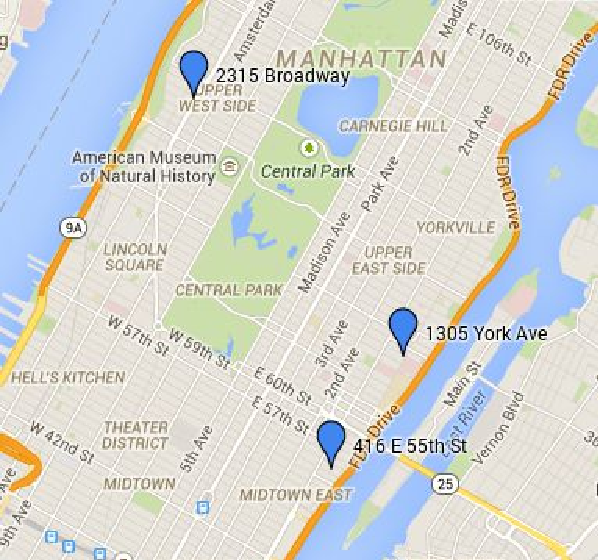
\includegraphics[scale=.6]{chap3/numeric/pic/site.pdf}
\caption{Locations of MRI facilities of New York Presbyterian. There
are three in total represented as blue bubbles. Two of them are on
the east side and one is on the west side.}
\label{fig:site}
\end{figure}

These sites have different numbers of MRI machines. West 84th has
only one machine. 55th St. has two machines. York Ave. has four machines.
Since they have different processing capacity, a different number of
appointments are scheduled for each. With 4 machines at York Ave, there is a
substantial amount of resource pooling ability present, making
patients there in general wait less.

The second scenario we consider is a system with 7 sites in which each has one
MRI machine. The reason is that we want to explore the impact of
diversion on a set of small cooperating imaging facilities. Also,
in this case, all sites are homogeneous, so we can isolate
the impact of resource pooling without worrying about imbalance between
processing capacities across sites.

\paragraph{Data}
We have three years of historical data for MRI scans at NYP Hospital.
For each of these scans, we have the type of scan, its appointment time, when
the patient arrived, when the scan began, and when the scan finished. The data we have
is not perfect, but we are able to fit reasonable model inputs based on it.

\begin{itemize}
\item Initial schedule for the day. We generate synthetic schedules
  where the number of scans of each type is proportional to the
  number of historical scans of that type.
\item The set of patients who are volunteers. We make the fraction
  of volunteers a parameter that varies across experiments.
  This can help us understand the amount of impact that diversions have
  with different levels of flexibility from patients.
\item Patient arrival time. We fit one empirical distribution on
  the difference between patient's arrival time and appointment time.
\item Preparation time. We do not actually have the timestamp data for this.
  We overcome this difficulty by considering the first patient processed each day,
  and use the difference between their arrival time and scan begin time
  as the preparation time. Since the first patient does not need to stay in the
  waiting room, it is reasonable to assume that all of the time between the arrival time
  and scan begin time is used for preparation. We fit one empirical distribution
  based on this.
\item Scan duration. For each type of scan, we fit an empirical
  scan duration distribution from historical data.
\item The set of SDAOPs and their arrival time. We calculate the rate of
  SDAOPs in the history and generate SDAOPs using a Possion process.
\item Cancellations. We calculate the historical probability of cancellation,
  and randomly select appointments that will be cancelled later.
\end{itemize}
Ideally, we would like to test our policy by replaying history with the real
scan duration and actual arrival time for each historical appointment. However,
the data we obtained is incomplete. There are some critical fields missing
and we cannot exactly reconstruct history. Furthermore, there are occasional
errors on timestamps that can greatly impact how the daily schedule appears.
To prevent these data issues from interfering with our experiments, we chose
to experiment with our constructed synthetic schedules.

One might improve the model inputs by predicting the scan duration and
arrival time better using more information. For example, the patient's
health condition, diagnosis, home address and other information might be
helpful to make a better prediction. However, we do not have access to these
sensitive personal data. But we believe that if we could use machine learning
techniques to make better predictions of patient's arrival time and scan duration,
our diversion policy would perform better.

\paragraph{Parameters}

There are several parameters we need to choose for setting up our simulation
and for our optimization procedure. We describe our choice of them here.

\begin{itemize}
  \item Volunteer probability. We vary the percent of patients who are willing
    to be volunteers. This will allow us to see the effect of our policy
    with varying levels of flexibility.
  \item Lead time. We experiment with both a 60 minute and a 90 minute lead time.
  \item Overtime weight $\lambda = 10$, this reflects the fact overtime is quite valuable.
  \item $\theta_c = 0.7, \theta_p = 0.7$. We choose the confidence threshold on objective value
    and waiting time of diverted patient to be neither too aggressive nor too conservative.
  \item The number of samples to evaluate quality of diversions $k=100$.
  \item The number of simulated days to estimate policy performance per experiment $k'=100$.
\end{itemize}
